\documentclass[final, usenames, dvipsnames]{beamer}
\mode<presentation>{\usetheme{GWU}}
\usepackage{poster_packages}
\usepackage{tikz_packages}
\tdplotsetmaincoords{60}{125} % view angle in spherical coordinates
\input{my_macros}

\DeclareSIUnit\year{yr}

\usepackage[orientation=landscape, width=121.92cm, height=91.44cm,scale=1.24,debug]{beamerposter} 
\beamertemplategridbackground[1cm] % grid for aligning stuff

%\setlength{\abovecaptionskip}{0.1cm}
%\setlength{\belowcaptionskip}{-0.3cm}

\def\newblock{} % Avoid the "\newblock undefined" error. See http://newsgroups.derkeiler.com/Archive/Comp/comp.text.tex/2008-07/msg00381.html"

%-----------------------------------------------------------
\newlength{\colsep}
\newlength{\onecolwidth}
\newlength{\twocolwidth}

\setlength{\paperwidth}{121.92cm} % 48in
\setlength{\paperheight}{91.44cm} % 36in


%\setlength{\onecolwidth}{0.23\textwidth} % Width of one column
%\setlength{\twocolwidth}{0.49\textwidth} % Width of two columns
\setlength{\onecolwidth}{28cm} % Width of one column
\setlength{\twocolwidth}{56cm} % Width of two columns
\newlength{\columnheight}
\setlength{\columnheight}{76.5cm}

\setbeamersize{text margin left=1.5cm,text margin right=0.5cm}

\listfiles

%-----------------------------
% MACROS
%-----------------------------
\def\Emph{\textcolor{RoyalBlue}}
%%%%%%%%%%%%%%%%%%%%%%%%%%%%%%%%%%%%%%%%%%%%%%%%%%%%%%%%%%%%%%%%%%%%%%%%%%%%%%%%%%%%%%
%	TITLE
%%%%%%%%%%%%%%%%%%%%%%%%%%%%%%%%%%%%%%%%%%%%%%%%%%%%%%%%%%%%%%%%%%%%%%%%%%%%%%%%%%%%%%%
\title{\Large Spacecraft Trajectory Design Near Asteroid 4769 Castalia}
\author{\Large \textcolor{white}{Shankar Kulumani}}
\institute{\large Flight Dynamics and Controls Laboratory (Dr. Taeyoung Lee)\\Department of Mechanical and Aerospace Engineering, School of Engineering and Applied Science}

%----------------------------------------------------------------------------------------

\begin{document}
\begin{frame}[t] % enclose entire poster in a frame
\begin{columns}[T,onlytextwidth] % start of all columns in poster

%-----------------------------------------------------------------------------------------
% FIRST (LEFT) COLUMN
%---------------------------------------------------------------------------------------
\begin{column}{\onecolwidth} % first column start

\begin{block}{Introduction} % Background block
	\begin{itemize}
		\item Asteroids and comets are of significant interest 
		\begin{itemize}
			\item \Emph{Science} - Insight into early solar system formation
			\item \Emph{Mining} - vast quantities of useful materials
			\item \Emph{Impact} - high risk from hazardous Near-Earth asteroids
		\end{itemize}
		\item Near-Earth asteroids (NEAs) are especially interesting 
		\begin{itemize}
			\item Orbit close to the Earth and are easily accessible
			\item Many asteroids hold vast quantities of useful materials
			\item Asteroid mining: Precious metals, propulsion fuels, semiconductors
			\item Commercialization is feasible with huge amounts of possible profit 
		\end{itemize}
		\item High probability of future asteroid impacts
	\end{itemize}
	\vspace{0.2in}
	\begin{figure}
        \begin{subfigure}[b]{0.4\columnwidth}%
	        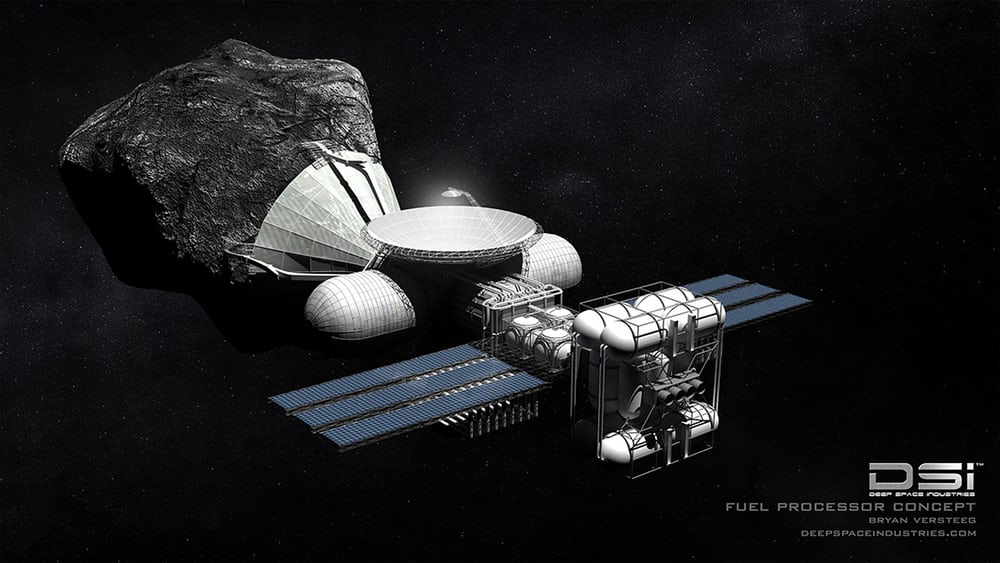
\includegraphics[height=8.5cm]{figures/asteroid-mining-feature-8.jpg}%
	        \caption*{Asteroid Mining}%
        \end{subfigure}~\hfill 
        \begin{subfigure}[b]{0.4\columnwidth}%
            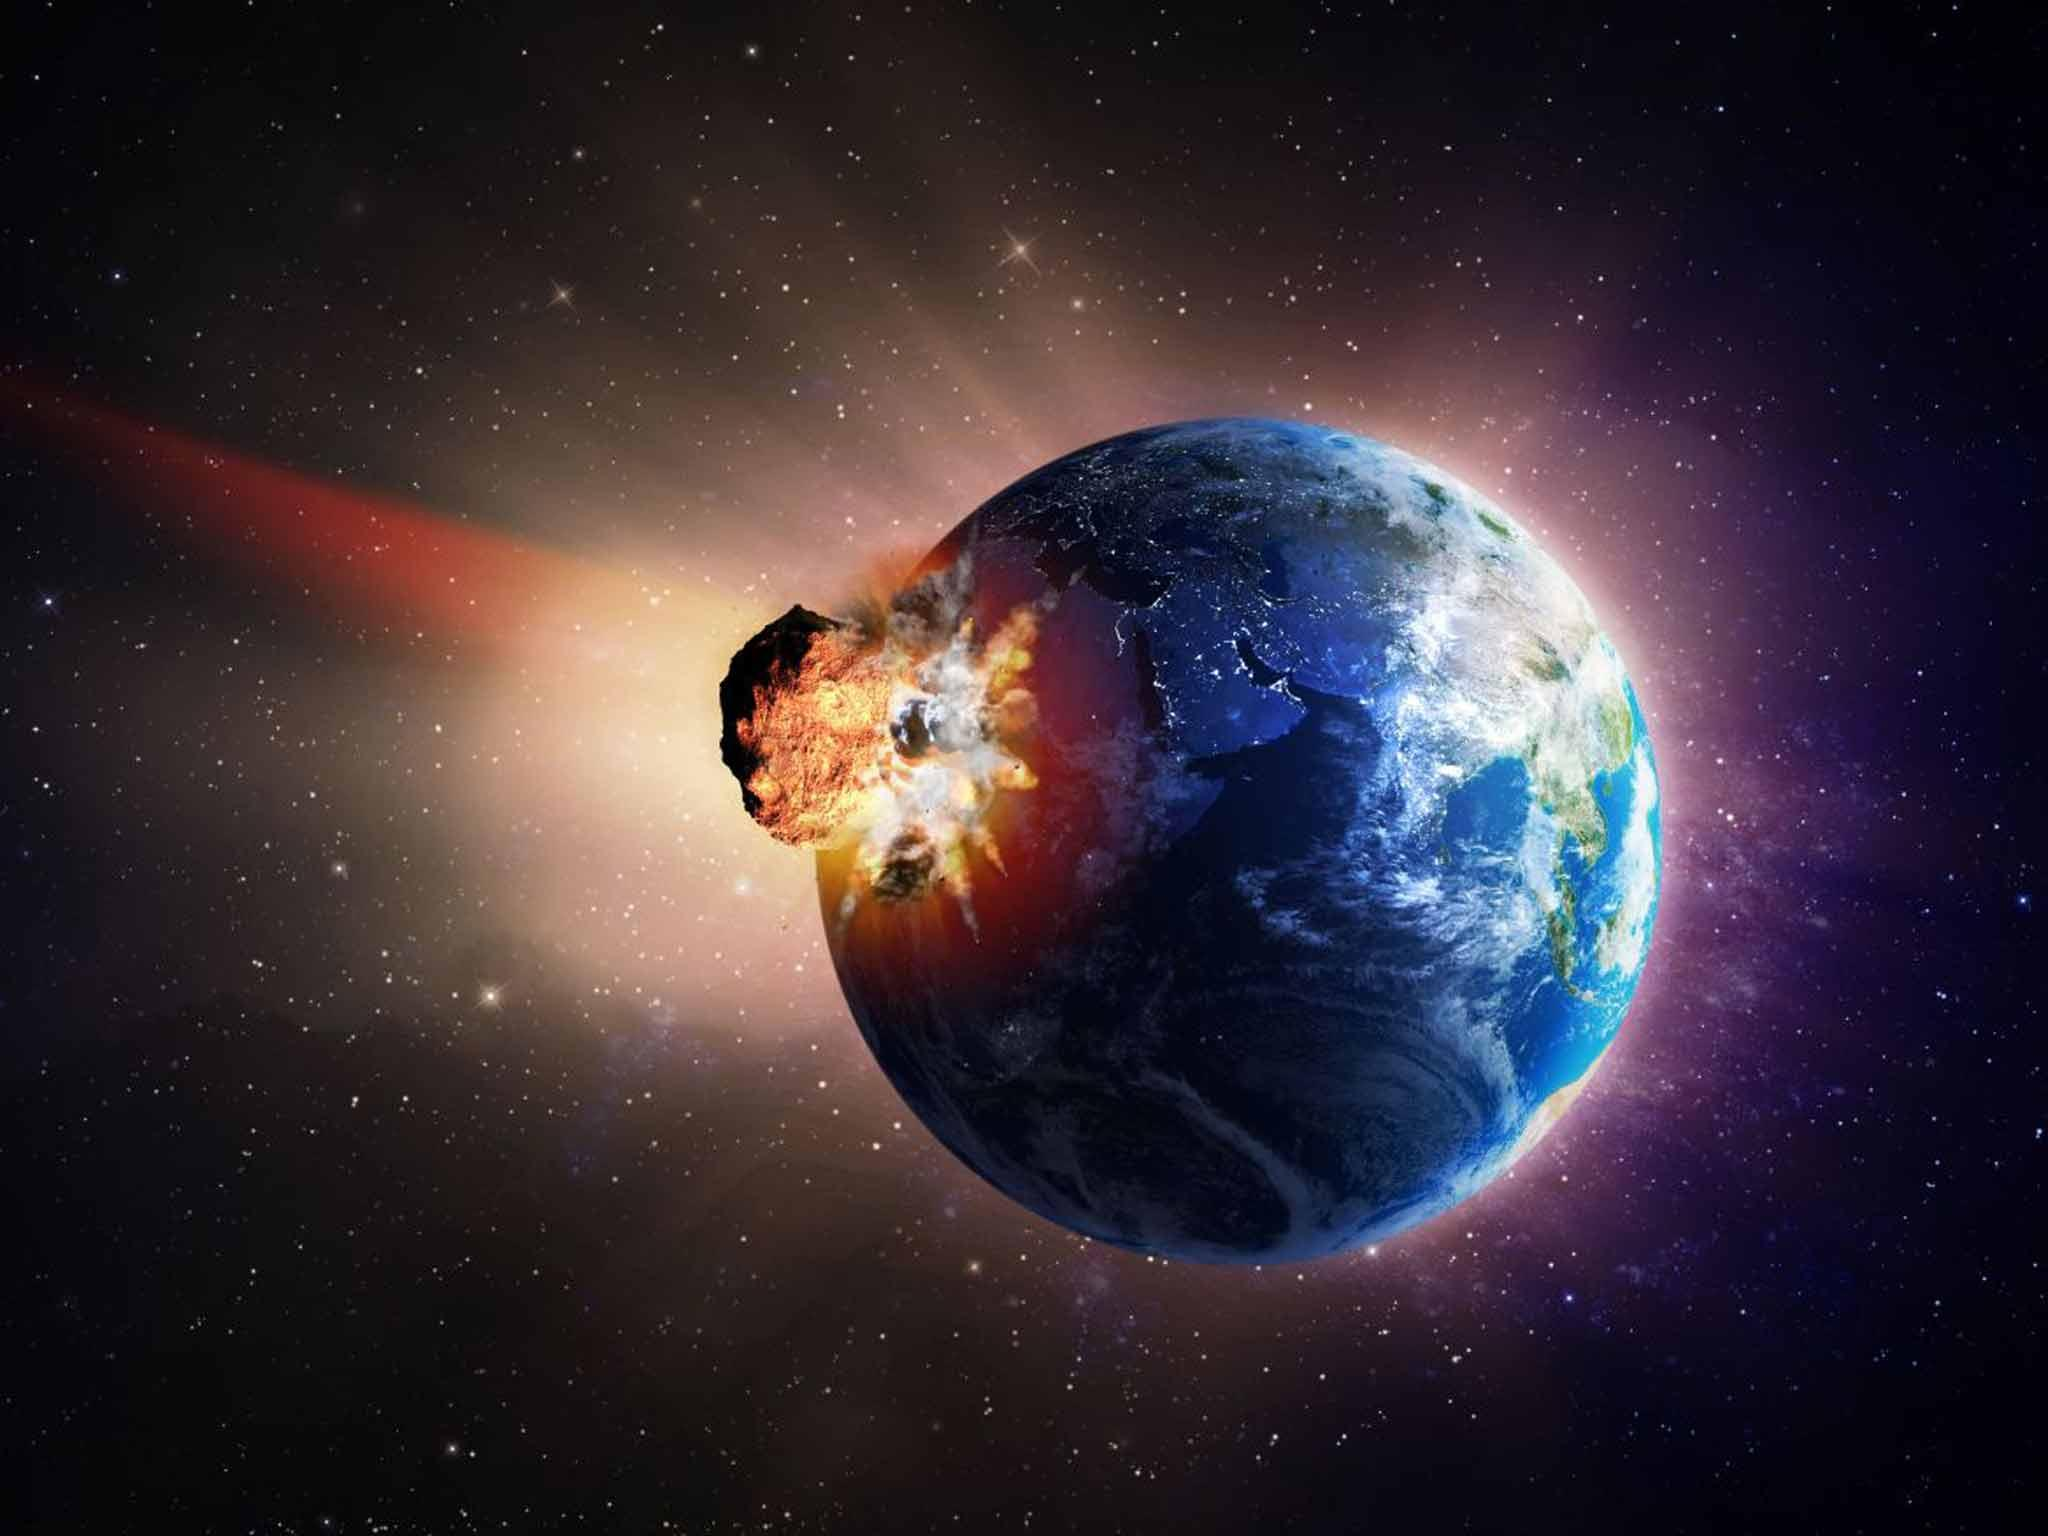
\includegraphics[height=8.5cm]{figures/asteroid-alamy.jpg}%
            \caption*{Asteroid Impact}%
        \end{subfigure}%
        \hfill%
	\end{figure}
\end{block} % end of background block

\begin{block}{Technical Challenges}
	\begin{itemize}
		\item Low-thrust propulsion systems offer innovative options
		\begin{itemize}
			\item Electric propulsion offers much greater efficiency
			\item Allows for greater velocity change with a reduced mass cost
			\item Key component for long duration missions with frequent thrusting
			\item Requires new methods of design
		\end{itemize}
		\item Optimal trajectory design is complicated
		\begin{itemize}
			\item Highly nonlinear and chaotic dynamics requires intuition by designer
			\item Using low-thrust propulsion adds additional difficulties in accurately capturing the small perturbations
		\end{itemize}
		\item Astrodynamic trajectory design typically uses direct optimal control
		\begin{itemize}
			\item Large nonlinear programming problem inherently approximates the true optimal solution
			\item High dimensionality of the solution makes it extremely computationally intensive
		\end{itemize}
	\end{itemize}
\end{block} 

\begin{block}{Gravitational Modeling}
	\begin{itemize}
		\item Asteroids are extended bodies - not point masses
		\begin{itemize}
			\item Gravity is the key force in orbital mechanics
			\item An accurate representation of gravity is critical to accurate and realistic analysis
		\end{itemize}
		\item Spherical Harmonic approach is popular but not ideal
		\begin{itemize}
			\item Model is only valid outside of circumscribing sphere
			\item Composed of an infinite series - always results in an approximation
			\item Model will diverge when close to the surface and is not ideal for landing missions
		\end{itemize}
		\item \Emph{Polyhedron Gravitational model} used to represent the asteroid
		\begin{itemize}
			\item Gravity is a function of the shape model
			\item Globally valid and closed-form analytical solution for gravity
			\item Exact potential assumes a constant density assumption
			\item Accuracy is only dependent on the shape
		\end{itemize}
	\end{itemize}
	\[
	U(\vecbf{r}) &= \frac{1}{2} G \sigma \sum_{e \in \text{edges}} \vecbf{r}_e \cdot \vecbf{E}_e \cdot \vecbf{r}_e \cdot L_e - \frac{1}{2}G \sigma \sum_{f \in \text{faces}} \vecbf{r}_f \cdot \vecbf{F}_f \cdot \vecbf{r}_f \cdot \omega_f 
	\]	
\end{block} 

\end{column}  % first column end

%-----------------------------------------------------------------------------------------
% SECOND (WIDE MIDDLE) COLUMN
%---------------------------------------------------------------------------------------
\begin{column}{\twocolwidth} % second column start

\begin{block}{Dynamics about the asteroid 4769 Castalia} % structure block
	\begin{minipage}{0.5\columnwidth} % left half of this block
	\begin{itemize}
		\item Dynamics are very similar to the famous three-body problem
			\[
			\begin{bmatrix} \dot{\vecbf{r}} \\ \dot{\vecbf{v}} \end{bmatrix} =
			\begin{bmatrix}\vecbf{v} \\ \vecbf{g} \parenth{\vecbf{r}} + \vecbf{h}\parenth{\vecbf{v}} + \vecbf{u} \end{bmatrix} 
			\]
		\item Huge history of analytical tools allow for great insight into the dynamics
		\item Analytical insight is critical to understanding the free motion around an asteroid
		\begin{itemize}
			\item We require an accurate understanding of the motion under the influence of gravity alone
			\item Efficient use of the limited oboard fuel is dependent on exploiting the natural dynamics of the asteroid environment
		\end{itemize}
		\item Jacobi Integral - single constant of motion which bounds the feasible regions in terms of ``energy''
			\[
			J \parenth{\vecbf{r}, \vecbf{v}} = \frac{1}{2} \omega^2 \parenth{x^2 + y^2} + U(\vecbf{r}) - \frac{1}{2} \parenth{\dot{x}^2 + \dot{y}^2 + \dot{z}^2} 
			\]
	\end{itemize}
	\end{minipage}% end of left half of block
	\begin{minipage}{0.5\columnwidth}% right half of block
		\begin{figure}
			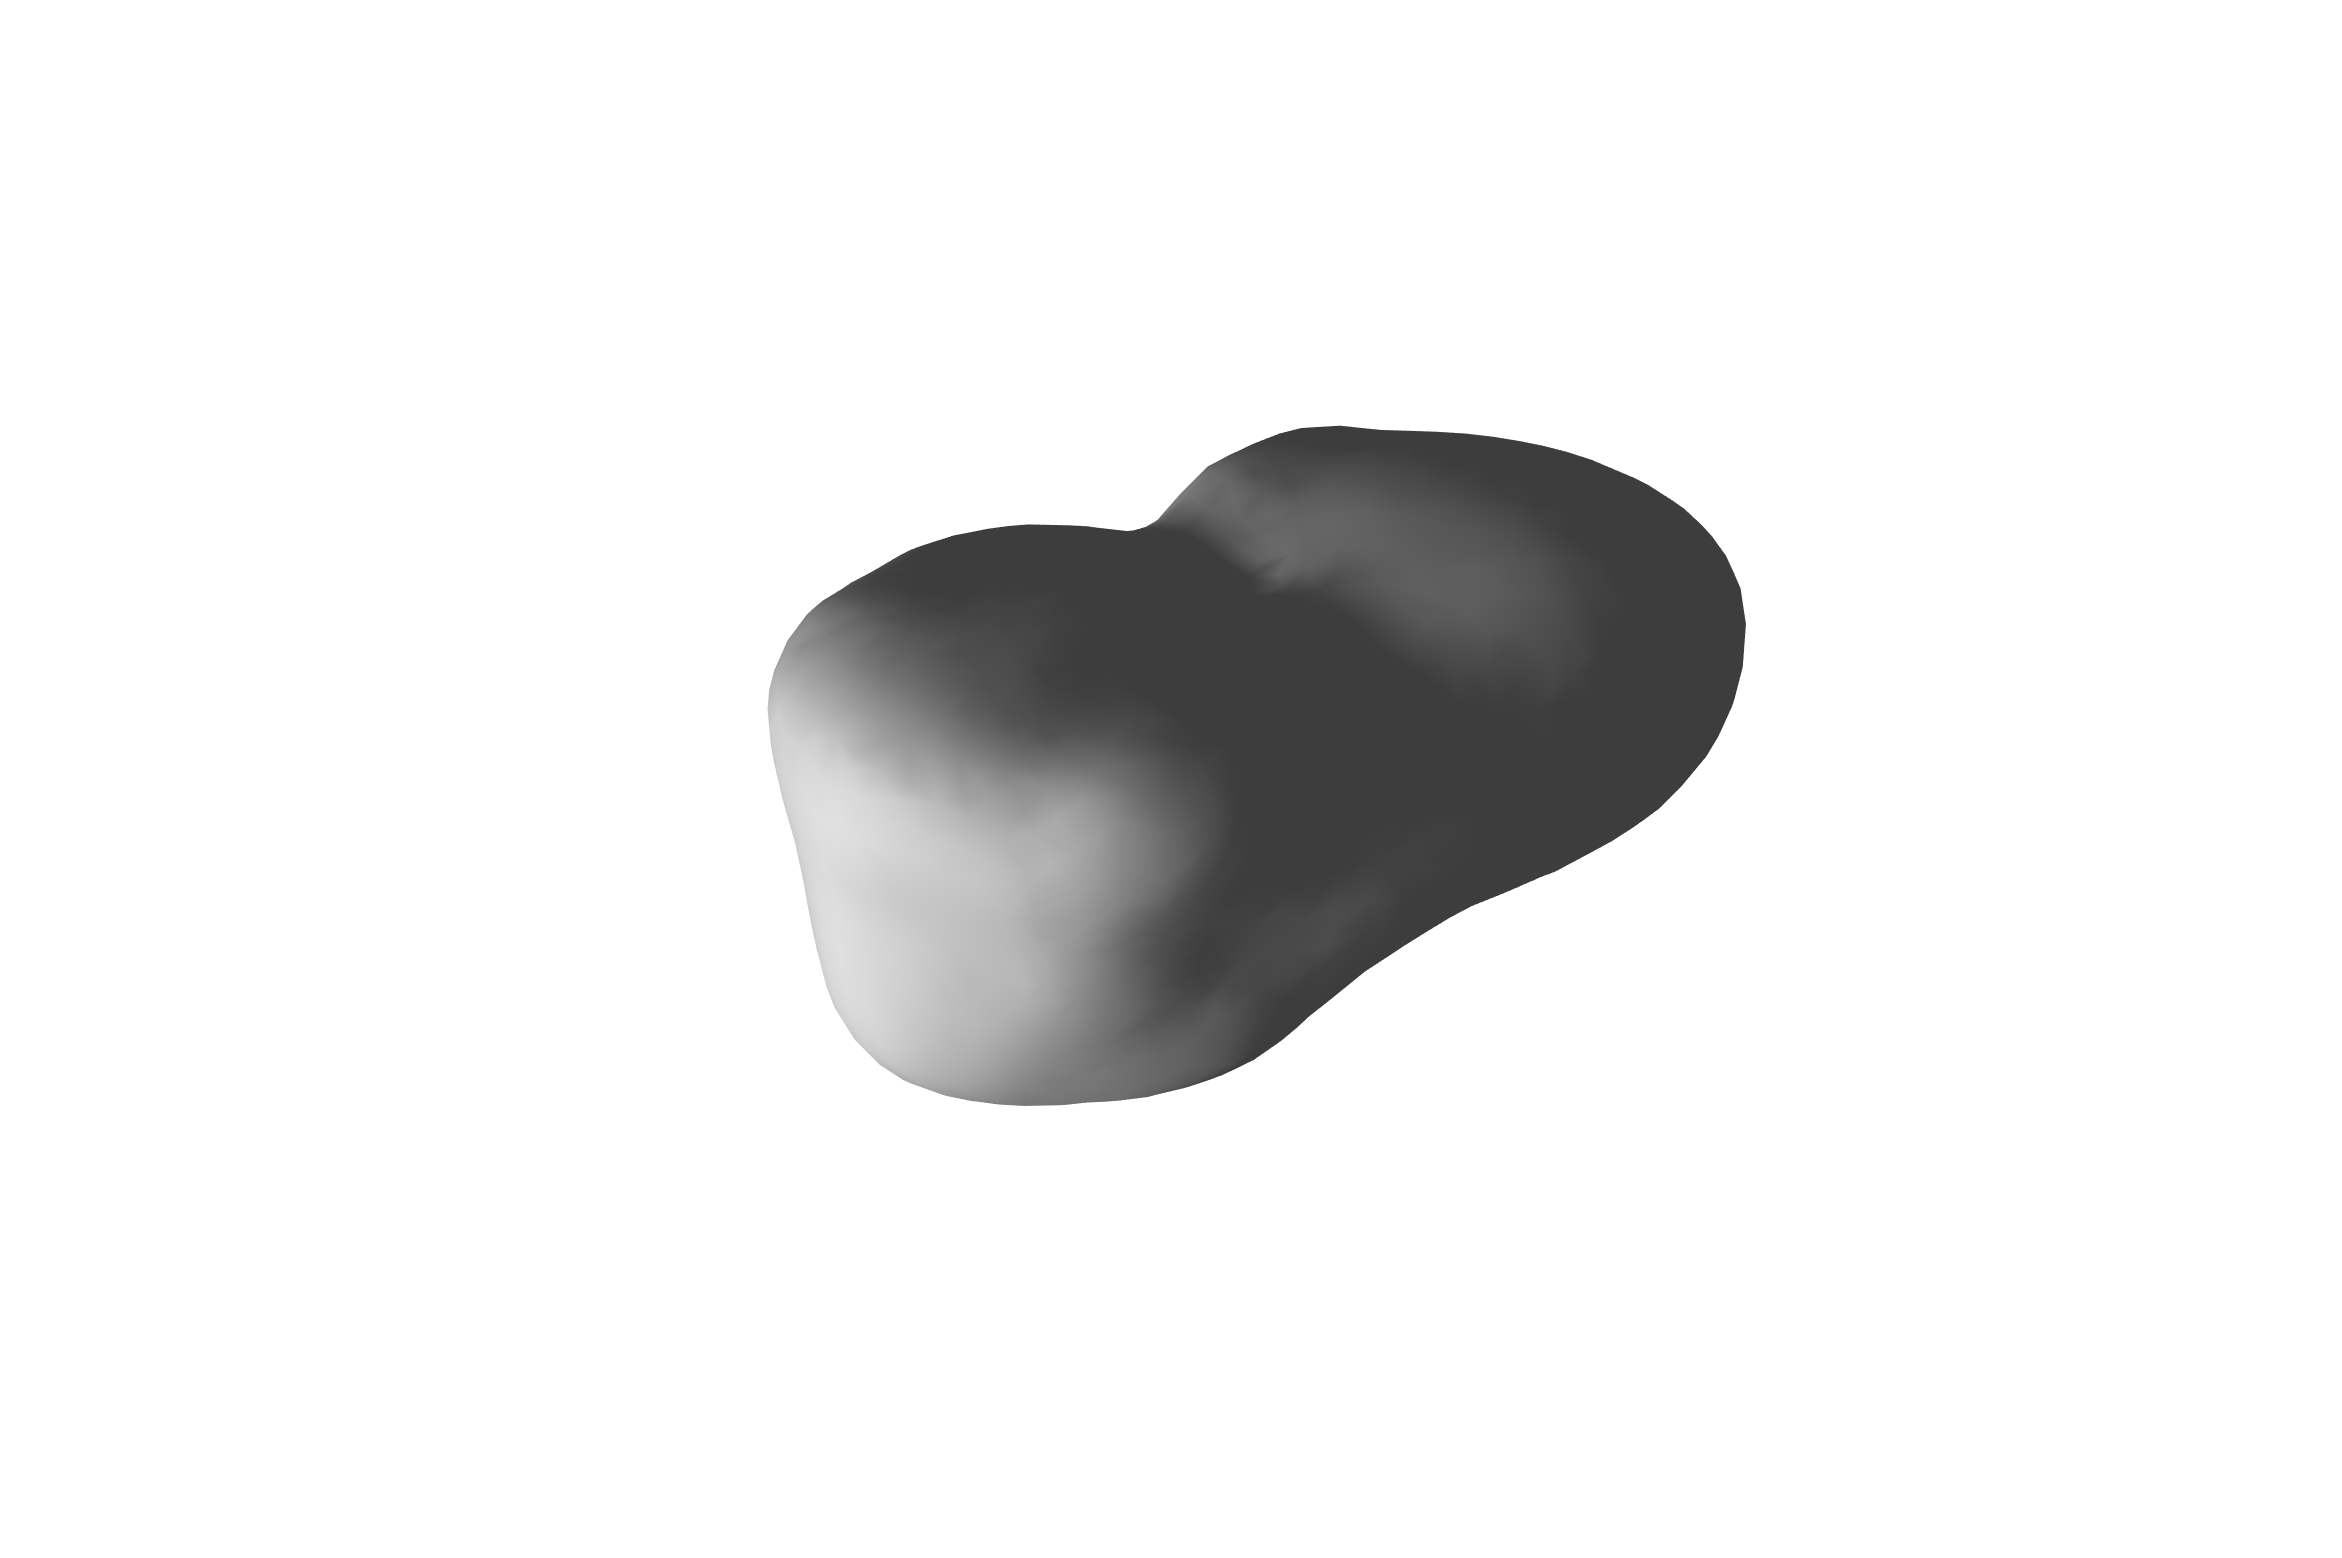
\includegraphics[trim={8cm 3cm 7cm 3cm},clip,width=\columnwidth]{figures/castalia.pdf}
			\caption*{Asteroid 4769 Castalia}
		\end{figure}
	\end{minipage}%end of right half of block
	
	\begin{itemize}
		\item All of this will span the width of the entire column.
		\item Since it is after the \texttt{minipage} environment
	\end{itemize}
\end{block} % end of structure block

\begin{block}{Reachability on the \Poincare section} % optimal control block

	\begin{figure}
	\centering
	\begin{scaletikzpicturetowidth}{0.5\columnwidth}
    \begin{tikzpicture}[tdplot_main_coords,
      poincare/.style={opacity=.2,very thick,fill=blue},
      orbit/.style={very thick,black},
      orbit hidden/.style={very thick,dashed},
      grid/.style={very thin,gray!50},
      axis/.style={->,blue,thick}, scale=\tikzscale]

    % nodes for the poincare section
    \node[label=above:\(\Sigma\)] (upper_right) at (0,5,5) {};
    \node[] (upper_left) at (0,1,5) {};
    \node[] (lower_left) at (0,1,0) {};
    \node[] (lower_right) at (0,5,0) {};

    % draw poincare section
    \draw[poincare] (upper_right.center) -- (upper_left.center) -- (lower_left.center) -- (lower_right.center) -- (upper_right.center);
    
    % draw a periodic orbit
    \coordinate (center) at (0,0,2);
    \node[below right] (x0) at (0,2,2) {\(\vecbf{q}_0\)};
    \filldraw (0,2,2) circle (3pt);

    \node[below right] (x1) at (0,3,2) {\(\vecbf{q}_1\)};
    \filldraw (0,3,2) circle (3pt);

    \tdplotdrawarc[orbit hidden]{(center)}{2}{90}{190}{}{};
    \tdplotdrawarc[orbit,<-]{(center)}{2}{-170}{90}{}{};

    \tdplotdrawarc[orbit hidden]{(center)}{3}{90}{199}{}{};
    \tdplotdrawarc[orbit,<-]{(center)}{3}{-161}{90}{}{};

	\end{tikzpicture}
    \end{scaletikzpicturetowidth}
	\caption{Diagram of the \Poincare map\label{fig:poincare_map}}
\end{figure}

\begin{figure}
	\centering
%	\includegraphics[width=0.5\textwidth]{reachability_set_hand}
	\begin{scaletikzpicturetowidth}{0.5\textwidth}
	\begin{tikzpicture}[tdplot_main_coords,
          poincare/.style={opacity=.2,very thick,fill=blue},
          orbit/.style={very thick,black},
          orbit hidden/.style={very thick,dashed},
          grid/.style={very thin,black},
          axis/.style={->,blue,thick},
          reachability/.style={thick,blue},scale=\tikzscale]

        % nodes for the poincare section
        \node[label=above:\(\Sigma\)] (upper_right) at (0,5,5) {};
        \node[] (upper_left) at (0,1,5) {};
        \node[] (lower_left) at (0,1,0) {};
        \node[] (lower_right) at (0,5,0) {};

        % draw poincare section
        \draw[poincare] (upper_right.center) -- (upper_left.center) -- (lower_left.center) -- (lower_right.center) -- (upper_right.center);
        
        % draw a periodic orbit
        \coordinate (center) at (0,0,2);
        \node[label=below:\(\vecbf{x}_n\)] (x0) at (0,3,2) {};
        % \node[label=below:\(\vecbf{x}_n\)] at (x0) {};
        \filldraw (x0) circle (3pt);

        % \tdplotdrawarc[orbit hidden]{(center)}{3}{90}{200}{}{};
        \tdplotdrawarc[orbit,<-]{(center)}{3}{-160}{90}{}{};

        % draw reachability set on the poincare section
        \coordinate (reach) at (0,4.5,2);
        \tdplotsetthetaplanecoords{90}

        \draw[tdplot_rotated_coords,grid] (x0) -- (reach);
        \draw[tdplot_rotated_coords,grid] (x0) -- ++(-45:1.5);

        \tdplotdrawarc[tdplot_rotated_coords,grid]{(x0)}{0.5}{-45}{90}{above}{\(\phi\)};

        % draw terminal state on reachability set
        \node[tdplot_rotated_coords,label=above:\(\vecbf{x}_f\)] (xf) at ($ (x0)+(-45:1.5) $) {};
        \filldraw (xf) circle (3pt);

        \node[tdplot_rotated_coords,label=below:\(J\)] at (xf) {};

        \tdplotdrawarc[tdplot_rotated_coords,reachability]{(x0)}{1.5}{0}{360}{}{};
        % place
    \end{tikzpicture}
	\end{scaletikzpicturetowidth}
	\caption{Reachability set on a \Poincare section\label{fig:reachability_set}}
\end{figure}

	\begin{itemize}
		\item \Emph{Spans the entire column width} 
		\begin{align*}
			\text{Initial: } R_0 =  \exp(\ang{225} \times \frac{\pi}{180} \hat{e}_3) \quad \text{Final: } R_d = I \quad \text{Disturbance: } \Delta = \begin{bmatrix} 0.2 & 0.2 & 0.2 \end{bmatrix}^T
		\end{align*}
		\item SCIENCE!
	\end{itemize}
\end{block} % end of optimal control block
\end{column}


%-----------------------------------------------------------------------------------------
% THIRD (RIGHT) COLUMN
%---------------------------------------------------------------------------------------
\begin{column}{\onecolwidth} % third column start

\begin{block}{Novel benefits} % results block
	\begin{itemize}
		\item Make sure to talk about how awesome your research is
	\end{itemize}
\end{block} % end of results block

\begin{block}{Conclusions} % conclusion
	\begin{itemize}
		\item Remind them about everything you already told them
		\item They should be quite amazed by this point
	\end{itemize}
\end{block} % conclusion
\end{column}  % third column end

\end{columns} % end of all columns in poster
\end{frame} % end of enclosing frame
\end{document}